\chapter{Superconductivity, Nambu Representation and Majorana Physics}

At the end of Session 4 we kept in mind the kind of fractionalization that we had built there, and
we pointed forward to a second example of it, which looks quite different. In a partially filled
topological flat band, correlations split the charge of the electron and make its exchange
statistics anyonic. In a superconductor, as we said there, pairing correlations instead split the
electron into two Majorana halves. In this session we will work out this second case in full. As
we will state carefully below, superconductors and fractional quantum Hall states are two
correlated states that both host fractional excitations, but through opposite mechanisms. The first
one has a mean-field description and needs an attractive interaction, and the second one has no
mean-field description and needs a strong repulsive interaction. The idea behind both is the same,
which is a correlated state with excitations that are not the electron itself, but the two routes
to it are really different. In this session we will build all the tools for the superconducting
route.

These tools also complete a topic that we left open before. In session 1 we built mean-field theory
as a general tool and then applied it quickly to three symmetry-broken states, a charge density
wave, a magnet and, as our third and shortest example, a superconductor. There we started from an
attractive Hubbard interaction and took an expectation value of two annihilation operators instead
of one creation and one annihilation operator. With this we defined the pairing order $\Delta =
\langle c_i c_j\rangle$ (session 1, eq. 1.9), and we showed that this term gets a phase
$e^{2i\varphi}$ under a gauge transformation, while every ordinary bilinear term stays invariant.
This means that a superconductor spontaneously breaks gauge symmetry, and with it the fixed electron
number. That first treatment was short on purpose. At that time we said that magnetism and
superconductivity would each get "a full, much deeper treatment in their own dedicated sessions
later in the course," and in this session it is the turn of superconductivity. Magnetism is moved
once more to the next recording, which is session 6 in the plan of this course.

So in this session we take up this topic again and build the full set of tools around it. First, we
need a new representation, the Nambu spinor, since without it we cannot even diagonalize a
Hamiltonian that mixes creation and annihilation operators in the way a pairing term does. This
representation gives us the Bogoliubov-de Gennes Hamiltonian, which is the central object of the
whole session. We will use it to classify superconducting order by symmetry, into singlet and
triplet and into s-, p- and d-wave. Then we will show that two superconductors can have the same
spectrum and still have a completely different topology, and to distinguish them we will use the
same Chern-number tools as in the topological-band-structure and quantum-Hall sessions. We will
follow this topological difference down to its strongest consequence, which is the Kitaev chain. We
will see that this model is the SSH model from the topological-band-structure session written in
terms of Majorana operators, and that its topological zero modes are their own antiparticles. At the
end we will ask what these Majorana modes can be used for, which is topological quantum computing.
We will also point to session 6, which does for magnetism what we are about to do for
superconductivity, and this is the one point of the course where the lecture explicitly leaves a
question open for the next recording. The same interacting Hamiltonian can give, at the mean-field
level, either a superconductor or a magnet, and magnetism is the topic that we moved to the next
recording.

\section{Weakly versus strongly correlated matter, revisited}

Before we specialize, let us state again the general setting, since it is useful to have it clearly
in mind. Every interacting Hamiltonian that we consider in this course has the same general form,

\begin{equation*}
H = \sum_{ij} t_{ij}\, c_i^\dagger c_j \;+\; \sum_{ijkl} V_{ijkl}\, c_i^\dagger c_j^\dagger c_k c_l,
\end{equation*}

which is a free bilinear part plus a quartic interaction, and it is exactly eq. 1.5 of session 1.
When mean-field theory can turn the quartic term into a good effective bilinear Hamiltonian, we call
the resulting state \emph{weakly correlated matter}. This includes magnets, charge density waves and
superconductors, which are all the states that we built in session 1. When no single-particle
mean-field Hamiltonian of this kind describes the physics, we have \emph{strongly correlated
matter}, and we need exact or numerical solutions instead. The fractional quantum Hall state from
the quantum-Hall session is our main example of this harder case.

Note that superconductors and the fractional quantum Hall state are at opposite ends of this
classification, even though both of them in the end host fractional excitations. A superconductor
has a mean-field description, comes from an \emph{attractive} interaction, is destroyed by a
magnetic field and, as we will see soon, hosts Majorana states. The fractional quantum Hall state
has no mean-field description, comes from strong \emph{repulsive} interactions, usually needs a
strong magnetic field and hosts excitations with fractional charge. Roughly speaking, both Majorana
excitations and fractional quantum Hall excitations are a fraction of an electron, but these
fractions come from completely different mechanisms. This is one of the good examples in this course
of how very different microscopic physics can lead to the same qualitative phenomenon, which is
emergent fractionalization, while the mechanism behind it is not the same at all.

\section{Superconductivity as a macroscopic quantum phenomenon}

Before we write the Hamiltonian, let us see why superconductivity is one of the clearest ways that
we have to observe quantum mechanics at the macroscopic scale. A superconductor is made of trillions
of atoms, and still a measurement on the bulk sample can give, essentially exactly, the microscopic
constants $\hbar$ and $e$. This works because gauge symmetry breaking gives the many-body wave
function a single well-defined phase $\theta(\mathbf{r})$, and the condition that this phase is
single-valued around a closed loop is a very strong constraint.

Let us take a superconducting ring threaded by magnetic flux, or in the same way a hole in a bulk
superconductor, and let us take the loop deep enough inside the superconductor that the
supercurrent density vanishes there because of Meissner screening. The supercurrent of Cooper pairs,
which have charge $2e$ since a pair is made of two electrons, is proportional to the gauge-invariant
combination $\hbar\nabla\theta -
2e\mathbf{A}$. If we set the current to zero on our loop, we obtain

\begin{equation*}
\oint \nabla\theta \cdot d\boldsymbol\ell = \frac{2e}{\hbar}\oint \mathbf{A}\cdot d\boldsymbol\ell = \frac{2e}{\hbar}\Phi.
\end{equation*}

However, $\theta$ is the phase of a single-valued wave function, so after one turn around the loop
it can only change by an integer multiple of $2\pi$, which means that $\oint \nabla\theta\cdot
d\boldsymbol\ell = 2\pi n$ for integer $n$. If we combine the two equations, we obtain flux
quantization,

\begin{equation}
\Phi = n\,\Phi_0, \qquad \Phi_0 = \frac{h}{2e}.
\end{equation}

Figure~\ref{fig:s05:flux} shows the geometry and the argument based on the winding of the phase.
The same physics is behind the precision of Josephson junctions. In the AC Josephson effect, a
voltage $V$ across the junction gives a current that oscillates with frequency $2eV/h$, which is a
direct macroscopic readout of $h/2e$, and this is possible only because gauge symmetry is broken. Note the parallel with the quantum Hall state from earlier in the course.
There, a macroscopic measurement also gives a ratio of the same two constants, which is the Hall
conductance, quantized in units of $e^2/h$ by the Chern number. However, the mechanism is completely
different, since it is the quantization of a single-particle topological invariant and not the
breaking of a continuous symmetry. In fact, if we combine the two measurements, the flux quantum and
the conductance quantum of the Hall effect, we have one of the most precise ways to obtain $h$ and
$e$ separately. This is a concrete example of the emergence that we keep coming back to in this
course, where macroscopic measurements on billions of atoms give us exact microscopic constants.

% Session 5 -- flux quantization as a macroscopic readout of h/2e.
% Placement: sec. "Superconductivity as a macroscopic quantum phenomenon", after eq. (5.1).
%
% LAYOUT NOTE: pure TikZ, no pgfplots axis, so every coordinate here is a canvas
% coordinate and nothing is positioned relative to an axis.
\begin{aqmfigure}{fig:s05:flux}{A drawing of flux quantization. On the left there is a superconducting
ring. Deep in the bulk the Meissner effect has already removed the supercurrent, so on the dashed
contour the gauge-invariant combination $\hbar\nabla\theta-2e\mathbf A$ vanishes and the phase
gradient is locked to the vector potential. On the right, when we move the condensate phase
$\theta$ once around this contour, it must come back to itself, so it can only wind by an integer
number of turns. Together, the two statements give $\Phi=n\,h/2e$, which means that the flux
through the hole is quantized, and the $2$ in the denominator is the charge $2e$ of a Cooper pair.
None of this is a property of a single electron. It is a macroscopic sample that gives back a ratio
of microscopic constants, only because gauge symmetry is broken.}

\begin{tikzpicture}[x=1cm, y=1cm]
\tikzset{
  gline/.style={aqm, draw=aqmmuted, line width=0.6pt, dash pattern=on 2pt off 1.5pt}
}

% ======================= (a) the ring ========================================
\node[aqmpanel, anchor=south] at (2.00,2.62) {(a) a ring, seen from above};

\begin{scope}[shift={(2.0,0.55)}]
  \fill[aqmfill, even odd rule] (0,0) circle(1.62) (0,0) circle(0.74);
  \draw[aqm, draw=aqmaccent] (0,0) circle(1.62);
  \draw[aqm, draw=aqmaccent] (0,0) circle(0.74);

  % flux through the hole: field out of the page
  \foreach \px/\py in {-0.34/-0.02, 0.34/-0.02, 0/-0.46} {
    \node[circle, draw=aqmbroken, line width=0.6pt, minimum size=6.5pt, inner sep=0pt]
      at (\px,\py) {};
    \fill[aqmbroken] (\px,\py) circle(0.85pt);
  }
  \node[aqmlabsmall, text=aqmbroken] at (0,0.36) {$\Phi$};

  % the contour, deep inside the superconductor
  \draw[aqm, draw=aqmbroken, dash pattern=on 3pt off 2pt,
        postaction={decorate, decoration={markings,
          mark=at position 0.16 with {\arrow{Stealth[length=5pt,width=4pt]}}}}]
    (0,0) circle(1.18);
\end{scope}

\node[aqmlabsmall, anchor=north, align=left, text width=4.55cm] at (2.00,-1.30)
  {\textcolor{aqmaccent}{shaded}: the superconductor\\[2pt]
   \textcolor{aqmbroken}{dashed}: a contour taken deep in the
   bulk, where Meissner screening has already made $J_s=0$\\[2pt]
   \textcolor{aqmbroken}{$\odot$}: the flux $\Phi$ through the hole};

% ======================= (b) the phase winds ==================================
\node[aqmpanel, anchor=south west] at (5.05,2.62)
  {(b) the phase, transported once around the contour};

\node[aqmlabsmall, anchor=south] at (5.45,2.00) {start};
\node[aqmlabsmall, anchor=south east, align=right] at (11.95,2.00)
  {same point, $\theta+2\pi$};

\foreach \i in {0,...,8} {
  \pgfmathsetmacro{\px}{5.45 + \i*0.80}
  \pgfmathsetmacro{\ang}{\i*45}
  \draw[aqm, draw=aqmmuted, line width=0.5pt] (\px,1.52) circle(0.27);
  \draw[aqm, draw=aqmaccent, -{Stealth[length=4pt,width=3.2pt]}]
    (\px,1.52) -- ++(\ang:0.27);
}
\draw[aqm, draw=aqmmuted, line width=0.5pt, -{Stealth[length=5pt,width=4pt]}]
  (5.45,1.08) -- (11.90,1.08);
\node[aqmlabsmall, text=aqmmuted, anchor=north] at (8.65,1.04)
  {once around the contour};

% the two constraints
\node[aqmlabsmall, anchor=west, align=left] at (5.05,0.24)
  {single-valued wave function:\quad
   $\displaystyle\oint\nabla\theta\cdot d\boldsymbol\ell = 2\pi n$};
\node[aqmlabsmall, anchor=west, align=left] at (5.05,-0.42)
  {no supercurrent on the contour:\quad
   $\displaystyle\oint\nabla\theta\cdot d\boldsymbol\ell = \frac{2e}{\hbar}\,\Phi$};

\node[aqmboxbroken, anchor=north west, font=\small] at (5.05,-0.95)
  {$\Phi = n\,\Phi_0,\qquad \Phi_0=\dfrac{h}{2e}$};

\node[aqmlabsmall, anchor=north west, align=left, text width=4.05cm, text=aqmbroken]
  at (9.75,-0.95) {the $2$ is the Cooper-pair charge; single electrons would give $h/e$};

% allowed flux ladder
\node[aqmlabsmall, anchor=west, text=aqmmuted] at (5.05,-2.55)
  {the only flux values the hole may carry:};
\draw[aqm, draw=aqmmuted, line width=0.5pt, -{Stealth[length=4pt,width=3pt]}]
  (5.45,-3.02) -- (11.90,-3.02);
\foreach \i/\lab in {0/$0$, 1/$\Phi_0$, 2/$2\Phi_0$, 3/$3\Phi_0$, 4/$4\Phi_0$} {
  \pgfmathsetmacro{\px}{5.75 + \i*1.42}
  \fill[aqmaccent] (\px,-3.02) circle(2.1pt);
  \node[aqmlabsmall, anchor=north] at (\px,-3.12) {\lab};
}

\end{tikzpicture}

\end{aqmfigure}


\section{Zero resistance and the Meissner effect in a superconductor}

In the history of the field, superconductivity was discovered through its transport signature. When
we cool an ordinary metal, the resistivity goes down smoothly, because there are fewer phonons from
which the electrons can scatter. A superconductor instead shows a \emph{sudden} drop of the
resistance to exactly zero at a critical temperature $T_c$. Below $T_c$ the resistance stays zero,
and not only small. $T_c$ is the temperature at which gauge symmetry breaking starts. This material
appears only on the slides and has no counterpart in the notebook. The schematic of the resistance
as a function of temperature and the figure of the field expulsion are shown and described on the
slides, but there is no notebook cell for them, since our companion notebook starts from the
Hamiltonian and not from transport measurements.

The second signature is the \textbf{Meissner effect}. Above $T_c$ a metal allows an external
magnetic field inside without any problem, but below $T_c$ the superconductor actively expels the
field from its bulk. In type-II superconductors, the only field that remains inside the material is
confined to quantized vortices, which are dynamical topological defects of the order parameter of
the broken gauge symmetry. Both signatures, zero resistance and the expulsion of the flux, are
direct consequences of the same event, which is the condensation of Cooper pairs into a single
macroscopic quantum state with a rigid phase that is chosen spontaneously.

\section{The interacting Hamiltonian and the origin of attractive interactions}

As in session 1, we start from the general interacting Hamiltonian $H = \sum_{ij}t_{ij}c_i^\dagger
c_j + \sum_{ijkl}V_{ijkl}c_i^\dagger c_j^\dagger c_k c_l$. The interaction $V_{ijkl}$ can come from
the plain electrostatic Coulomb repulsion, which is repulsive, but it can also be an
\emph{effective} interaction mediated by another quasiparticle in the material. Examples are
phonons, which are lattice vibrations, magnons, which are fluctuations of a magnetic moment,
plasmons, which are collective charge fluctuations, and even more exotic mediators such as skyrmion
fluctuations or valence fluctuations. For superconductivity, what matters is not the microscopic
origin of $V_{ijkl}$ but its net sign in the channel that turns out to be relevant, and
superconductivity requires this channel to be effectively \emph{attractive}.

This is the natural point to distinguish the two families of superconductors.

\begin{itemize}
\item \textbf{Conventional superconductors}, where the attractive channel is mediated by phonons.
  This is the case that we understand best. Mean-field theory, which is called BCS theory, works
  well at the quantitative level, and the critical temperatures of simple conventional
  superconductors such as aluminum or lead can be predicted from theory.
\item \textbf{Unconventional superconductors}, where the attraction is mediated by anything that is
  not a phonon, such as antiferromagnetic or ferromagnetic magnons, plasmons, valence fluctuations,
  charge fluctuations and others. Here we do not have a predictive theory that is equally reliable.
  Even to identify \emph{which} quasiparticle mediates the attraction in a given unconventional
  superconductor is often still an open research question, and it is one of the major unsolved
  problems that the field is working on today.
\end{itemize}

\section{The mean-field pairing Hamiltonian in detail}

Let us now build the mean-field pairing Hamiltonian with the same care that we used in session 1 for
the charge-density-wave and magnetic examples, instead of only pointing at $\Delta = \langle
cc\rangle$. We take the simplest interacting Hamiltonian that can give superconductivity, which is a
one-dimensional tight-binding chain with an attractive onsite interaction between opposite spins,

\begin{equation}
H = -t\sum_{n,\sigma}\left(c_{n\sigma}^\dagger c_{n+1,\sigma} + \text{h.c.}\right) - \mu\sum_{n\sigma}c_{n\sigma}^\dagger c_{n\sigma} + U\sum_n c_{n\uparrow}^\dagger c_{n\downarrow}^\dagger c_{n\downarrow} c_{n\uparrow}, \qquad U<0.
\end{equation}

This is exactly eq. 1.7 of session 1, now with $U = -|U| < 0$. It is the attractive branch of the
same Hamiltonian, and its repulsive branch gives rise to magnetism, which is the topic of session 6.
This time we do the mean-field decoupling of the quartic term in the \emph{pairing} channel, also
called the particle-particle channel, instead of the density channel. We define the order parameter

\begin{equation}
\Delta_n \equiv U\langle c_{n\downarrow}c_{n\uparrow}\rangle,
\end{equation}

and we factorize $c_{n\uparrow}^\dagger c_{n\downarrow}^\dagger c_{n\downarrow}c_{n\uparrow} \approx
\langle c_{n\uparrow}^\dagger c_{n\downarrow}^\dagger\rangle c_{n\downarrow}c_{n\uparrow} +
c_{n\uparrow}^\dagger c_{n\downarrow}^\dagger \langle c_{n\downarrow}c_{n\uparrow}\rangle - \langle
c_{n\uparrow}^\dagger c_{n\downarrow}^\dagger\rangle\langle c_{n\downarrow}c_{n\uparrow}\rangle$.
This is the same Wick-type factorization that we used in all of session 1, now applied to a
different pair of operators. The resulting mean-field Hamiltonian is

\begin{equation}
H_{\text{MF}} = -t\sum_{n\sigma}\left(c_{n\sigma}^\dagger c_{n+1,\sigma}+\text{h.c.}\right) - \mu\sum_{n\sigma}c_{n\sigma}^\dagger c_{n\sigma} + \sum_n\left(\Delta_n\, c_{n\uparrow}^\dagger c_{n\downarrow}^\dagger + \Delta_n^*\, c_{n\downarrow}c_{n\uparrow}\right) - \sum_n\frac{|\Delta_n|^2}{U}.
\end{equation}

When we solve it self-consistently, $\Delta_n$ is exactly zero for $U>0$, the repulsive case, and it
can become nonzero for $U<0$, the attractive case. This is the superconducting order parameter, and
it is the term that breaks gauge symmetry.

\begin{notebookbox}{\texttt{session5.ipynb}, ``s-wave superconductivity driven by attractive interactions'' (Core), and ``Dependence on the strength of the attractive interaction'' (Challenge)}
Build the attractive-Hubbard chain of (5.2), run the pairing self-consistency loop that gives
$\Delta$ in (5.3)-(5.4), and look at how $\Delta$ grows from zero as you make $U$ more negative.
This is the same behavior as in session 1, where the charge imbalance grew with $V$ and the
magnetization grew with $U>0$.
\end{notebookbox}

\section{Why pairing does not conserve the particle number}

Let us now show in an exact way the statement from session 1 that the electron number fluctuates,
instead of only stating it. We take the eigenvalue equation $H_{\text{MF}}|G\rangle = E|G\rangle$
for the Hamiltonian in (5.4), and we expand the ground state in the occupation-number basis, which
is the Fock basis, ordered by the total particle number $N$, as $|G\rangle = \sum_N a_N |N\rangle$.
The hopping and chemical-potential terms in (5.4) conserve $N$ exactly, since each of them has one
$c^\dagger$ and one $c$. The pairing terms $\Delta_n
c_{n\uparrow}^\dagger c_{n\downarrow}^\dagger$ and $\Delta_n^* c_{n\downarrow}c_{n\uparrow}$ change
$N$ by $+2$ and $-2$ respectively. The key point is that \emph{no term in $H_{\text{MF}}$ ever
changes $N$ by $\pm 1$}. So $H_{\text{MF}}$ only connects Fock states whose particle numbers differ
by an even integer. For $|G\rangle$ to be an eigenstate, $a_N$ can then be nonzero only inside one
fixed parity class of $N$, either all even or all odd. However, this says nothing about which even
or odd values of $N$ appear, and in general $a_N \ne 0$ for several values of $N$ in that class,
for example $N=0,2,4,\dots$ at the same time. The mean-field ground state is therefore \emph{not}
an eigenstate of the total number operator $\hat N$, even though it has a well-defined fermion
parity. This is the exact meaning of the statement that a superconductor has a fluctuating electron
number but a fixed parity, which session 1 pointed out in its discussion of the superposition
puzzle of the quantum dot (session 1, section 1.5).

\section{The gauge transformation in explicit form}

We already wrote the gauge transformation in second quantization in session 1 (eq. 1.10), $c \to
c\, e^{i\varphi}$, $c^\dagger \to c^\dagger e^{-i\varphi}$. It is the second-quantized version of
the statement that the phase of a first-quantized wave function has no physical meaning. Let us now
check explicitly which terms of a realistic Hamiltonian stay invariant under this transformation and
which do not. Ordinary hopping $c_i^\dagger c_j$ is invariant, since the two phases cancel, as
$c_i^\dagger c_j \to
e^{-i\varphi}c_i^\dagger \cdot e^{i\varphi} c_j = c_i^\dagger c_j$. The same cancellation protects
essentially every other bilinear term that we have seen so far, such as magnetic terms that depend
on spin, spin-orbit coupling and any density-density interaction term $c_i^\dagger c_i c_j^\dagger
c_j$, because all of them are built from the same number of creation and annihilation operators,
which pair up index by index.

The pairing term is the only exception. Under the same transformation,

\begin{equation}
\Delta\, c_{n\uparrow}^\dagger c_{n\downarrow}^\dagger \;\longrightarrow\; \Delta\, e^{-2i\varphi}\, c_{n\uparrow}^\dagger c_{n\downarrow}^\dagger,
\end{equation}

it gets the phase \emph{twice}, because both operators are creation operators and not one creation
and one annihilation operator. No choice of $\varphi \ne 0 \pmod \pi$ leaves this term invariant, so
a Hamiltonian with a nonzero $\Delta$ is not gauge invariant term by term. In an equivalent way, if
we write the transformation as acting on the order parameter itself, $\Delta \to \Delta\,
e^{2i\varphi}$, then any fixed phase of $\Delta$ is a choice that the ground state makes
spontaneously, which is the signature of continuous symmetry breaking. This is the same logic that
session 1 used to show the gauge symmetry breaking of eq. 1.9, now applied in full detail, and we
have now seen why the factor is $2\varphi$ and not $\varphi$.

\section{The Nambu spinor and the Bogoliubov-de Gennes Hamiltonian}

The pairing term creates a technical problem. We cannot diagonalize (5.4) with an ordinary vector of
orbital operators, because the anomalous term mixes creation and annihilation operators, instead of
pairing them up in the way of every Hamiltonian that we diagonalized in sessions 1-4. The solution
is to \emph{enlarge} the operator basis, so that both the creation and the annihilation operators of
the original problem become entries of a bigger spinor that behave like annihilation operators. We
work in momentum space, with a single orbital and both spins, and we define the \textbf{Nambu
spinor}

\begin{equation}
\Psi_{\mathbf{k}} = \begin{pmatrix} c_{\mathbf{k}\uparrow} \\ c_{\mathbf{k}\downarrow} \\ c_{-\mathbf{k}\downarrow}^\dagger \\ -c_{-\mathbf{k}\uparrow}^\dagger \end{pmatrix},
\end{equation}

which has an electron sector, formed by the first two components and containing
ordinary annihilation operators, and a hole sector, formed by the last two components and
containing creation operators at $-\mathbf{k}$, with the spins exchanged and with an extra minus sign
on the last entry. This sign has a real role. It is what is needed so that, when we write
$H_{\text{MF}}$ in terms of $\Psi_{\mathbf k}$, the pairing term gives two identical and decoupled
copies of the same $2\times 2$ problem, instead of mixing the two spin blocks through a Pauli
matrix. For a spin-singlet pairing $\Delta(\mathbf k)$, which does not depend on momentum and is
equal to $\Delta$ for the Fourier transform of the onsite case of (5.4), one can check directly,
using the fermionic anticommutation relations to reorder operators where needed, that the
mean-field Hamiltonian can be written exactly as

\begin{equation}
H_{\text{MF}} = \frac{1}{2}\sum_{\mathbf{k}} \Psi_{\mathbf{k}}^\dagger\, H_{\text{BdG}}(\mathbf{k})\, \Psi_{\mathbf{k}} + \text{const.}, \qquad H_{\text{BdG}}(\mathbf{k}) = \begin{pmatrix} \varepsilon(\mathbf{k}) & 0 & \Delta(\mathbf k) & 0 \\ 0 & \varepsilon(\mathbf k) & 0 & \Delta(\mathbf k) \\ \Delta(\mathbf k)^* & 0 & -\varepsilon(\mathbf{k}) & 0 \\ 0 & \Delta(\mathbf k)^* & 0 & -\varepsilon(\mathbf k) \end{pmatrix},
\end{equation}

where $\varepsilon(\mathbf k) = -2t(\cos k_x + \cos k_y) - \mu$ is the ordinary band dispersion,
which we assume to be inversion symmetric, $\varepsilon(-\mathbf k) = \varepsilon(\mathbf k)$. This
$4\times 4$ matrix is called the \textbf{Bogoliubov-de Gennes (BdG) Hamiltonian}, and in a concrete
sense it is the most important object to describe the excitations of a superconductor. Note that
the two diagonal entries in the lower-right part have $-\varepsilon(\mathbf k)$ and not
$+\varepsilon(\mathbf k)$. This comes directly from writing $c_{-\mathbf k\sigma}^\dagger
c_{-\mathbf k\sigma}$ in terms of $c_{-\mathbf k\sigma}c_{-\mathbf k\sigma}^\dagger = 1 -
c_{-\mathbf k\sigma}^\dagger c_{-\mathbf
k\sigma}$ with the anticommutation relations. This is also where the name hole comes from, since a
missing electron at $-\mathbf k$ behaves like a particle with opposite energy.

Since the spinor (5.6) was built with this extra minus sign, the $4\times 4$ problem in (5.7) is
already block-diagonal. There is one $2\times 2$ block built from $(c_{\mathbf k\uparrow},
c_{-\mathbf k\downarrow}^\dagger)$ and an identical one built from $(c_{\mathbf k\downarrow},
-c_{-\mathbf
k\uparrow}^\dagger)$, and each of them has the reduced BdG matrix

\begin{equation}
h_{\text{BdG}}(\mathbf k) = \begin{pmatrix} \varepsilon(\mathbf k) & \Delta(\mathbf k) \\ \Delta(\mathbf k)^* & -\varepsilon(\mathbf k)\end{pmatrix}.
\end{equation}

This is the structure that is shown on the slides and quoted in the lecture, a $4\times 4$ matrix
for a single orbital with two spins, with diagonal entries $\varepsilon(\mathbf k)$,
$\varepsilon(\mathbf k)$, $-\varepsilon(\mathbf k)$,
$-\varepsilon(\mathbf k)$
and off-diagonal entries $\Delta$, but now we have derived it instead of only stating it. If we
diagonalize (5.8), we obtain the standard BCS quasiparticle dispersion

\begin{equation}
E(\mathbf k) = \pm\sqrt{\varepsilon(\mathbf k)^2 + |\Delta(\mathbf k)|^2}.
\end{equation}

\begin{notebookbox}{\texttt{session5.ipynb}, ``Nambu electronic structure without superconductivity'' and ``Nambu electronic structure with superconductivity'' (both Reminder)}
First build the Nambu-doubled Hamiltonian of (5.6)-(5.7) with $\Delta = 0$, and check that you get
exactly two copies of the same band structure. One is the physical copy, which is the electron
sector, and the other is a spurious mirror copy, which is the hole sector, with dispersion
$-\varepsilon(\mathbf k)$. Then turn on $\Delta$ and look at how the gap in (5.9) opens at every
crossing between the two copies.
\end{notebookbox}

\section{An example of a gap that opens independently of the dispersion}

Equation (5.9) already tells us something that the slides of the lecture show with explicit band
plots. The gap opens at the minimum of $E(\mathbf k)$, which is where $\varepsilon(\mathbf
k) = 0$, that is, exactly on the original Fermi surface, and the minimum gap there is
$|\Delta(\mathbf
k)|$ evaluated on that Fermi surface. Nothing in this argument depends on the details of
$\varepsilon(\mathbf k)$, such as the range of the hopping, the lattice geometry or the position of
the chemical potential. For concreteness, let us take the single-orbital square lattice with
$\varepsilon(\mathbf k) =
\cos k_x + \cos k_y$ (units where $t=1$) and a chemical potential such that the physical red band
and the spurious blue mirror band cross. When we turn on a constant $\Delta$, a gap of size
$2|\Delta|$ opens at every such crossing, for \emph{any} choice of the chemical potential along this
dispersion. The same statement holds if we do the calculation on the triangular lattice instead of
the square lattice. As we move the chemical potential across the band of the triangular lattice, a
uniform $\Delta$ still opens a gap everywhere the physical and the spurious bands cross. This is the
general signature of \emph{conventional} superconductivity, which is fully gapped, since a uniform
$\Delta(\mathbf k)$ that does not depend on momentum always gaps the whole Fermi surface,
regardless of the microscopic details.

\begin{notebookbox}{\texttt{session5.ipynb}, ``Superconductivity, full spectral function and electron spectral function'' (Core), and ``The impact of superconductivity in an electronic structure'' (Challenge)}
Reproduce the square-lattice example above. Plot the spectral function of the electron sector with
$\Delta = 0$, where there are two crossing copies, and then with $\Delta \ne 0$, where a gap of size
$2|\Delta|$ opens at the crossing, as in eq. 5.9. Repeat this for the triangular-lattice dispersion
and check that the gap opens regardless of where you put the chemical potential.
\end{notebookbox}

\section{Metal, gapped and nodal superconductor for one Fermi surface}

Not every pairing function $\Delta(\mathbf k)$ is independent of momentum, and this gives more
interesting cases. For a given electronic dispersion $\varepsilon(\mathbf k)$ there are in general
three qualitatively different outcomes.

\begin{enumerate}
\item \textbf{No superconductivity} ($\Delta = 0$). This is a metal, which is gapless everywhere on
the Fermi surface.
\item \textbf{Conventional (s-wave) superconductivity.} Here $\Delta(\mathbf k) \ne 0$ everywhere on
the Fermi surface, so $E(\mathbf k)$ in (5.9) stays away from zero everywhere, and there is a full
gap.
\item \textbf{Unconventional, nodal superconductivity.} Here $\Delta(\mathbf k)$ vanishes along some
lines or points of the Brillouin zone. Wherever the Fermi surface crosses one of these nodal lines,
$E(\mathbf
k) = 0$ even though $\Delta \ne 0$ nearby. The system is gapped in most of reciprocal space, but it
stays gapless, which means metallic, at isolated momenta or along nodal lines.
\end{enumerate}

% Session 5 -- the three scenarios for one Fermi surface: metal, gapped SC, nodal SC.
% Placement: sec. "Three scenarios for one Fermi surface", after the enumerated list.
% Rendered by figures/blender/s05f02_fsgap.py, labels in figures/overlays/s05f02_fsgap.tex.
\begin{aqmfigure}{fig:s05:fsgap}{One Fermi surface with three outcomes. Each panel shows the
Brillouin zone with a small Fermi pocket around $\Gamma$, and the height of the tube standing on the
pocket is the minimum of the quasiparticle energy $E(\mathbf k)=\sqrt{\varepsilon(\mathbf
k)^2+|\Delta(\mathbf k)|^2}$ as we go once around it. Since $\varepsilon=0$ on the Fermi surface,
this minimum is $|\Delta|$ evaluated there, which is why the pairing function only matters \emph{on}
the Fermi surface. (a) Without pairing the whole pocket is at zero energy, which is a metal. (b) A
constant $\Delta_0$ lifts every point of it by the same amount, which gives a full gap. (c) The
$d$-wave gap (5.13) vanishes on the zone diagonals, the red lines, and the pocket crosses them in
four places, so four gapless points survive in a superconductor that is gapped everywhere else.
Nodes in other parts of the zone do not appear in the spectrum, and only nodes that intersect the
Fermi surface give gapless quasiparticles.}
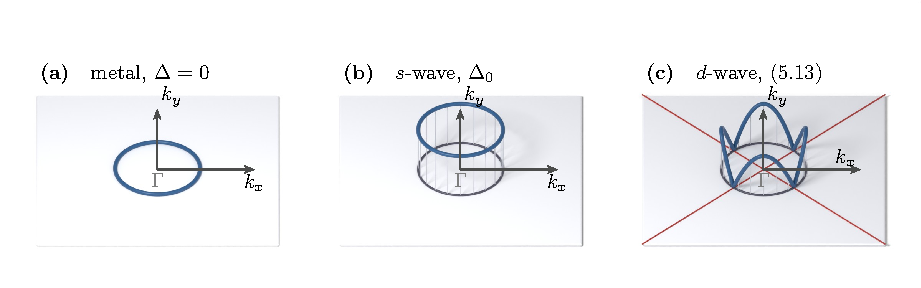
\includegraphics{figures/pdf/s05f02_fsgap.pdf}
\end{aqmfigure}


Figure~\ref{fig:s05:fsgap} shows the three cases next to each other, in the Brillouin zone and also
as the gap along the Fermi surface itself, which is the only place where the gap can be read at all.
The high-temperature cuprate superconductors are the standard example of scenario 3 in real
materials. They are real superconductors, but their gap function has nodes, so parts of their Fermi
surface stay gapless even in the superconducting state. This division into three cases holds for
any lattice geometry, and the lecture shows it explicitly for the Fermi surfaces of both the square
and the triangular lattice.

\begin{notebookbox}{\texttt{session5.ipynb}, ``Unconventional singlet superconducting orders'' (Challenge), and ``Gapped and nodal superconducting orders'' (Core)}
Build a $\Delta(\mathbf k)$ that depends on momentum and vanishes along a line in the Brillouin
zone, for example the d-wave form of section 5.12 below. Then check numerically with (5.9) that the
gap closes exactly where the Fermi surface crosses this nodal line, which is different from the
uniformly gapped case of section 5.9.
\end{notebookbox}

\section{The general pairing Hamiltonian and its symmetry classification}

Up to now $\Delta$ has been a single number. In general the pairing order can depend on momentum and
have a spin structure, $\Delta_{\mathbf k,\sigma_1\sigma_2}$ with $\sigma_1,\sigma_2 \in
\{\uparrow,\downarrow\}$. We can write it in a compact way as the $2\times 2$ pairing matrix
$\Delta_{\mathbf
k} = \begin{pmatrix}\Delta_{\mathbf k,\uparrow\uparrow} & \Delta_{\mathbf k,\uparrow\downarrow}\\
\Delta_{\mathbf k,\downarrow\uparrow} & \Delta_{\mathbf k,\downarrow\downarrow}\end{pmatrix}$, and
it is built from a general mean-field Hamiltonian

\begin{equation}
H_{\text{pair}} = -\frac{1}{2}\sum_{\mathbf k}{}^{\prime}\, \sum_{\sigma_1\sigma_2} \left[\Delta_{\mathbf k,\sigma_1\sigma_2}\, c_{\mathbf k\sigma_1}^\dagger c_{-\mathbf k\sigma_2}^\dagger + \Delta_{\mathbf k,\sigma_1\sigma_2}^*\, c_{\mathbf k\sigma_1} c_{-\mathbf k\sigma_2}\right],
\end{equation}

The real-space and reciprocal-space pictures of $\Delta$ are related by a Fourier transform, so we
can also think of this order in terms of how the pair wave function looks as a function of the
distance between the two paired electrons in real space. The key step is to classify
superconducting order only by the \emph{symmetry} of $\Delta_{\sigma\sigma'}(\mathbf k)$, because
this symmetry alone controls how the superconductor responds to perturbations, such as disorder or
magnetic fields, independently of the microscopic details.

Fermionic antisymmetry, which comes from the fact that the operators $c_{\mathbf k\sigma}^\dagger
c_{-\mathbf k\sigma'}^\dagger$ anticommute, imposes

\begin{equation}
\Delta_{\sigma\sigma'}(\mathbf k) = -\Delta_{\sigma'\sigma}(-\mathbf k),
\end{equation}

which is a minus sign under the \emph{combined} operation of exchanging the spin indices and sending
$\mathbf k \to
-\mathbf k$. This combined statement holds for any type of pairing. The classification that has a
physical meaning comes from splitting $\Delta_{\sigma\sigma'}(\mathbf k)$ into a part that is
symmetric and a part that is antisymmetric under spin exchange alone. Because of (5.11), this is the
same as splitting it by its parity under $\mathbf k \to -\mathbf k$ alone,

\begin{equation*}
\textbf{Spin singlet (even parity):} \quad \Delta(\mathbf k) = \Delta(-\mathbf k), \qquad \Delta_{\sigma\sigma'} = -\Delta_{\sigma'\sigma}\ \text{(spin-antisymmetric)},
\end{equation*}
\begin{equation}
\textbf{Spin triplet (odd parity):} \quad \Delta(\mathbf k) = -\Delta(-\mathbf k), \qquad \Delta_{\sigma\sigma'} = +\Delta_{\sigma'\sigma}\ \text{(spin-symmetric)}.
\end{equation}

For concreteness, onsite s-wave pairing, with $\Delta(\mathbf k) = \Delta$ constant, which comes
from a local attractive interaction as in section 5.5, is even in $\mathbf k$, and so it is
spin-singlet. This symmetry classification has a direct physical consequence. A spin-singlet
superconductor is essentially insensitive to non-magnetic disorder, which is called Anderson's
theorem, since the pair wave function only depends on time-reversed partners, and non-magnetic
disorder preserves them. A spin-triplet superconductor, on the other hand, is strongly suppressed
even by weak non-magnetic disorder, because scattering mixes the different momentum directions
between which the order parameter needs to keep coherent phase relations. This is the reason why
spin-singlet s-wave superconductors are much more common in nature than spin-triplet ones.
Essentially every real material has some level of non-magnetic disorder, and this disorder destroys
the triplet channel and leaves the singlet channel intact.

\section{Building a spin-triplet superconductor out of a magnet}

Since spin-triplet order is so fragile, how could we ever build one on purpose? One way is a toy
model that has both a ferromagnetic exchange field and an attractive interaction in the same
Hamiltonian,

\begin{equation*}
H = -t\sum_{\langle ij\rangle,\sigma}c_{i\sigma}^\dagger c_{j\sigma} \;\underbrace{-\, h\sum_i \left(c_{i\uparrow}^\dagger c_{i\uparrow} - c_{i\downarrow}^\dagger c_{i\downarrow}\right)}_{\text{exchange field}} \;+\; \underbrace{U\sum_{\langle ij\rangle} c_{i\sigma}^\dagger c_{j\sigma'}^\dagger c_{j\sigma'}c_{i\sigma}}_{\text{attractive interaction}}, \qquad U<0.
\end{equation*}

If we solve it self-consistently at the mean-field level, both order parameters, the ferromagnetic
exchange field and the pairing amplitude, can be nonzero at the same time. The ground state then
breaks both time-reversal symmetry, since it is magnetic, \emph{and} gauge symmetry, since it is
superconducting. The pairing that survives is necessarily spin-triplet, because the exchange field
explicitly splits the $\uparrow$ and $\downarrow$ Fermi surfaces, and in this way it suppresses the
singlet channel, which needs them to be degenerate. Physically, s-wave singlet pairing is usually
the leading instability because it can gap the \emph{entire} Fermi surface, which gives the largest
condensation energy. When the exchange field suppresses this channel, a different pairing channel
becomes the leading instability instead, which here is the odd-parity, spin-triplet channel, which
is effectively p-wave.

The most interesting feature of this state appears when we put it on a finite ribbon instead of an
infinite plane. The bulk spectrum is gapped, as we expect for a superconductor, but the edges of the
ribbon have gapless excitations. A superconductor that is fully gapped in the bulk and gapless at
the edge is a signature that we already know from the topological-band-structure and quantum-Hall
sessions. Indeed, these edge modes have a topological origin, and they are tied to a finite Chern
number of the underlying BdG band structure, in the same way as the edge states of a Chern
insulator were tied to its Chern number.

\begin{notebookbox}{\texttt{session5.ipynb}, ``The impact of a spin splitting in an electronic structure'' (Reminder), ``A spin triplet superconductor'' (Core), ``Majorana modes in a spin triplet superconductor'' (Challenge), ``Interaction-induced spin-triplet superconductivity'' (Challenge), and ``Topological modes in interaction-driven spin triplet superconductors''}
Start from the plain spin-split band structure, with only an exchange field, to build intuition.
Then run the self-consistency loop for the model above and check that a spin-triplet $\Delta$
emerges. Move to a ribbon geometry and find the gapless edge modes described here, and then, in the
later challenge sections of the notebook, connect them to the Majorana physics of sections
5.15-5.17.
\end{notebookbox}

\section{Nodal singlet order, d-wave pairing in the cuprates and the angular-momentum expansion}

Inside the spin-singlet, even-parity order there is a further useful distinction, since a singlet
gap can be uniformly nonzero, as in the s-wave case of section 5.9, or it can be nodal. The standard
example of the second case is \textbf{d-wave} order on the square lattice,

\begin{equation}
\Delta_{d}(\mathbf k) = \Delta_0\left(\cos k_x - \cos k_y\right),
\end{equation}

which vanishes exactly along the diagonals of the Brillouin zone, $k_x = \pm k_y$. Together with
(5.9), this means that the quasiparticle spectrum $E(\mathbf k) = \sqrt{\varepsilon(\mathbf k)^2 +
\Delta_d(\mathbf k)^2}$ is gapless where the Fermi surface crosses these diagonals, which gives a
nodal singlet superconductor. This is the pairing symmetry of the cuprate high-temperature
superconductors, which have critical temperatures up to about 130 K at ambient pressure, above the boiling
point of liquid nitrogen, and are spin-singlet, but clearly \emph{not} s-wave.

Behind this there is a clear and general way to organize the possible cases, which is analogous to
the expansion of an atomic orbital wave function in spherical harmonics. We expand the
superconducting gap in an angular-momentum basis on the Fermi surface,

\begin{equation}
\Delta(\mathbf k) \;\sim\; \sum_L \Delta_L\, Y_L(\mathbf k),
\end{equation}
\begin{equation*}
\begin{aligned}
L=0:\quad &\text{s-wave (conventional, typically phonon-driven)},\\
L=1:\quad &\text{p-wave (spin-triplet, often ferromagnetic-magnon-driven)},\\
L=2:\quad &\text{d-wave (spin-singlet, often antiferromagnetic-magnon-driven; cuprates)}.
\end{aligned}
\end{equation*}

In real and reciprocal space, s-wave order is flat and constant, with no momentum dependence at
all. The $d_{x^2-y^2}$ order of (5.13) changes sign around the Fermi surface in a pattern of four
lobes, $+,-,+,-$, with the same name and the same lobe structure as an atomic $d$ orbital. There is
also a third possibility, which is called \emph{extended s-wave}. It is still $L=0$, meaning that it
has the same overall symmetry as plain s-wave under the lattice point group, but it is nodal along
the \emph{radial} direction, since it is positive near the zone center $\Gamma$, goes through a
node and is negative further out. Figure~\ref{fig:s05:gapsymmetry} shows these sign structures over
the Brillouin zone, together with the p- and f-wave cases below.

The lecture repeats the same classification into three cases, uniform s-wave, a nodal order and
extended s-wave, on the triangular lattice. There the nodal case has six lobes of alternating sign
around the Fermi surface, and it is an \textbf{f-wave order, $L=3$}. The instructor confirmed this,
and the "L equal to two" in the raw recording was a mistake, since a pattern of six lobes with
alternating sign is the standard signature of $L=3$ and not of $L=2$, which is already used above
for the four-lobed $d_{x^2-y^2}$ state of the square lattice. Note that this order is outside the
singlet family of this section. Six lobes with alternating sign mean that the gap changes sign under
a half turn, so $\Delta(-\mathbf k) =
-\Delta(\mathbf k)$, and by (5.12) an $L=3$ order has odd parity and is therefore necessarily
\emph{spin-triplet}, and not singlet like the s-, extended-s- and d-wave cases above.

% Session 5 -- the angular-momentum classification of the pairing function.
% Placement: sec. "Nodal singlet order: d-wave, cuprates, and the angular-momentum expansion",
% after the extended-s-wave paragraph.
%
% What each panel shows is the SIGN of Delta(k) over the Brillouin zone, with the nodal
% lines dashed. The parity under k -> -k (i.e. under a point reflection of the panel through
% its centre) is then something the reader can read off by eye, and (5.12) converts it
% immediately into singlet or triplet. Panels (a)-(d) are the square lattice, panel (e) the
% triangular lattice with its hexagonal zone.
\begin{aqmfigure}{fig:s05:gapsymmetry}{The sign structure of $\Delta(\mathbf k)$ over the Brillouin
zone, ordered by angular momentum $L$ as in (5.14), where the dashed lines are the nodes. A
reflection of a panel through its centre sends $\mathbf k\to-\mathbf k$. Panels with even $L$ do
not change and are therefore spin singlets, and panels with odd $L$ come back with every sign
flipped and are spin triplets, which is (5.12) seen in a picture. Counting lobes is the fastest
way to identify the order. Two lobes mean $L=1$, four mean $L=2$ and six mean $L=3$, and any
pattern whose lobes alternate an odd number of times in a half turn is necessarily odd in
$\mathbf k$, so it is a triplet. This is why the $f$-wave state (e), which has six lobes, is a
spin triplet, even though it is similar to the singlet $d$-wave state in every other respect.
Extended $s$-wave (b) deserves a second look, since its node is radial and not angular. It has the
same even parity and the same point-group symmetry as plain $s$-wave, and only the position of its
node ring relative to the Fermi surface decides whether it is nodal in the spectrum. The overall
sign of $\Delta$ is a gauge choice, and only the sign \emph{changes} are physical.}

\begin{tikzpicture}[x=1cm, y=1cm]
\tikzset{
  nodeline/.style={aqm, draw=aqmbroken, line width=0.8pt, dash pattern=on 3pt off 2pt},
  bzbox/.style={aqm, draw=black, line width=\aqmthinwidth},
  plus/.style={aqmlabsmall, text=aqmaccent},
  minus/.style={aqmlabsmall, text=aqmbroken}
}
\def\B{0.98}     % half-width of the square Brillouin zone
\def\Hx{1.06}    % circumradius of the hexagonal zone

% ============================ (a) s-wave =====================================
\begin{scope}[shift={(1.35,0)}]
  \fill[aqmfill] (-\B,-\B) rectangle (\B,\B);
  \draw[bzbox] (-\B,-\B) rectangle (\B,\B);
  \node[plus] at (0,0) {$+$};
  \node[aqmpanel, anchor=south] at (0,\B+0.10) {(a) $s$};
  \node[aqmlabsmall, anchor=north, align=center, text width=2.5cm] at (0,-\B-0.12)
    {$\Delta_0$\\[1pt]$L=0$, even\\[-1pt]\textcolor{aqmaccent}{singlet}};
\end{scope}

% ============================ (b) extended s-wave ============================
\begin{scope}[shift={(4.30,0)}]
  \fill[aqmfillb] (-\B,-\B) rectangle (\B,\B);
  \fill[aqmfill] (-\B,0) -- (0,\B) -- (\B,0) -- (0,-\B) -- cycle;
  \draw[bzbox] (-\B,-\B) rectangle (\B,\B);
  \draw[nodeline] (-\B,0) -- (0,\B) -- (\B,0) -- (0,-\B) -- cycle;
  \node[plus] at (0,0) {$+$};
  \node[minus] at (0.68,0.68) {$-$};
  \node[minus] at (-0.68,-0.68) {$-$};
  \node[aqmpanel, anchor=south] at (0,\B+0.10) {(b) ext.\ $s$};
  \node[aqmlabsmall, anchor=north, align=center, text width=2.5cm] at (0,-\B-0.12)
    {$\cos k_x+\cos k_y$\\[1pt]$L=0$, even\\[-1pt]\textcolor{aqmaccent}{singlet}};
\end{scope}

% ============================ (c) p-wave =====================================
\begin{scope}[shift={(7.25,0)}]
  \fill[aqmfillb] (-\B,-\B) rectangle (0,\B);
  \fill[aqmfill] (0,-\B) rectangle (\B,\B);
  \draw[bzbox] (-\B,-\B) rectangle (\B,\B);
  \draw[nodeline] (0,-\B) -- (0,\B);
  \draw[nodeline] (-\B,-\B) -- (-\B,\B);
  \draw[nodeline] (\B,-\B) -- (\B,\B);
  \node[plus] at (0.50,0) {$+$};
  \node[minus] at (-0.50,0) {$-$};
  \node[aqmpanel, anchor=south] at (0,\B+0.10) {(c) $p$};
  \node[aqmlabsmall, anchor=north, align=center, text width=2.5cm] at (0,-\B-0.12)
    {$\sin k_x$\\[1pt]$L=1$, odd\\[-1pt]\textcolor{aqmbroken}{triplet}};
\end{scope}

% ============================ (d) d-wave =====================================
\begin{scope}[shift={(10.20,0)}]
  \fill[aqmfillb] (0,0) -- (\B,\B) -- (\B,-\B) -- cycle;
  \fill[aqmfillb] (0,0) -- (-\B,\B) -- (-\B,-\B) -- cycle;
  \fill[aqmfill] (0,0) -- (-\B,\B) -- (\B,\B) -- cycle;
  \fill[aqmfill] (0,0) -- (-\B,-\B) -- (\B,-\B) -- cycle;
  \draw[bzbox] (-\B,-\B) rectangle (\B,\B);
  \draw[nodeline] (-\B,-\B) -- (\B,\B);
  \draw[nodeline] (-\B,\B) -- (\B,-\B);
  \node[minus] at (0.62,0) {$-$};
  \node[minus] at (-0.62,0) {$-$};
  \node[plus] at (0,0.62) {$+$};
  \node[plus] at (0,-0.62) {$+$};
  \node[aqmpanel, anchor=south] at (0,\B+0.10) {(d) $d$};
  \node[aqmlabsmall, anchor=north, align=center, text width=2.5cm] at (0,-\B-0.12)
    {$\cos k_x-\cos k_y$\\[1pt]$L=2$, even\\[-1pt]\textcolor{aqmaccent}{singlet}};
\end{scope}

% ============================ (e) f-wave, triangular lattice =================
\begin{scope}[shift={(13.30,0)}]
  \foreach \i in {0,2,4} {
    \pgfmathsetmacro{\a}{\i*60}
    \pgfmathsetmacro{\b}{\a+60}
    \fill[aqmfill] (0,0) -- (\a:\Hx) -- (\b:\Hx) -- cycle;
  }
  \foreach \i in {1,3,5} {
    \pgfmathsetmacro{\a}{\i*60}
    \pgfmathsetmacro{\b}{\a+60}
    \fill[aqmfillb] (0,0) -- (\a:\Hx) -- (\b:\Hx) -- cycle;
  }
  \draw[bzbox] (0:\Hx) -- (60:\Hx) -- (120:\Hx) -- (180:\Hx) -- (240:\Hx) -- (300:\Hx) -- cycle;
  \foreach \i in {0,1,2} {
    \pgfmathsetmacro{\a}{\i*60}
    \draw[nodeline] (\a:\Hx) -- ({\a+180}:\Hx);
  }
  \foreach \i in {0,2,4} {
    \pgfmathsetmacro{\a}{\i*60+30}
    \node[plus] at (\a:0.62) {$+$};
  }
  \foreach \i in {1,3,5} {
    \pgfmathsetmacro{\a}{\i*60+30}
    \node[minus] at (\a:0.62) {$-$};
  }
  \node[aqmpanel, anchor=south] at (0,\B+0.10) {(e) $f$};
  \node[aqmlabsmall, anchor=north, align=center, text width=2.6cm] at (0,-\B-0.12)
    {triangular lattice\\[1pt]$L=3$, odd\\[-1pt]\textcolor{aqmbroken}{triplet}};
\end{scope}

\end{tikzpicture}

\end{aqmfigure}


\begin{notebookbox}{\texttt{session5.ipynb}, ``Gapped and nodal superconducting orders'' (Core)}
Implement the $d_{x^2-y^2}$ gap of (5.13) on the square lattice, plot $\Delta(\mathbf k)$ over the
Brillouin zone, and check the pattern of four lobes with alternating sign and the position of its
nodes relative to a given Fermi surface. The nodal $L=3$ (f-wave) case of the triangular lattice
discussed above is also in this section of the notebook, if you want to see the pattern of six
lobes directly.
\end{notebookbox}

\section{Same gap and different topology in trivial s-wave and chiral p-wave pairing}

This is the central point of the whole session. Two superconducting gaps can have completely
identical \emph{spectral} properties, where both fully gap the Fermi surface with, for example, the
same minimum gap, and still be topologically different. Let us compare plain s-wave pairing,
$\Delta(\mathbf k) =
\Delta_0$, with \textbf{chiral p-wave} pairing,

\begin{equation}
\Delta_{p+ip}(\mathbf k) = \Delta_0\left(\sin k_x + i \sin k_y\right),
\end{equation}

which is an odd-parity, spin-triplet order, in agreement with (5.12) since $\Delta_{p+ip}(-\mathbf
k) =
-\Delta_{p+ip}(\mathbf k)$, and which winds once around the origin of the complex plane as $\mathbf
k$ goes around the Fermi surface. Both (5.9) with $\Delta_0$ and (5.9) with $\Delta_{p+ip}$ can
fully gap the same Fermi surface, so a measurement of the bulk gap alone cannot distinguish them.
However, in the same way as for the Chern-number classification of gapped bands in the
topological-band-structure session, we can compute the Chern number of the occupied BdG bands for
each case, and the two results are completely different. The trivial s-wave state has Chern number
$0$, while the chiral p-wave state has Chern number $\pm 2$, where the sign is set by the
chirality, $p_x + ip_y$ or $p_x - ip_y$.

What distinguishes them, as shown in figure~\ref{fig:s05:topology}, is the winding of the
\emph{phase} of $\Delta(\mathbf k)$ when $\mathbf k$ goes once around the Fermi surface. This phase
is constant for s-wave, and it makes one full turn for $p+ip$.

This has the consequence that we expect from the bulk-boundary correspondence. In a finite system,
the s-wave superconductor stays gapped everywhere, both in the bulk and at the edge, in the same way
as a trivial insulator with Chern number zero. The chiral p-wave superconductor, on the other hand,
is gapped in the bulk but has gapless \emph{chiral} edge modes. On one edge there are $|C|$ branches
that all propagate in the same direction, here two, one from each of the two identical spin blocks,
and the opposite edge has the same number of branches that propagate in the opposite direction, as
a state with Chern number $\pm 2$ must have. So on a ribbon we see two sets of branches that
propagate in opposite directions, but they are localized on opposite edges and do not share one
edge. These edge modes turn out to be fractions of an electron in a very specific and exact sense,
since they are Majorana modes, and the rest of this session is about what this means.

% Session 5 -- same gap, different topology: trivial s-wave versus chiral p-wave.
% Placement: sec. "Same gap, different topology", after the bulk-boundary paragraph.
% Rendered by figures/blender/s05f04_topology.py, labels in figures/overlays/s05f04_topology.tex.
\begin{aqmfigure}{fig:s05:topology}{Two gaps that a spectroscopy experiment cannot distinguish, seen
from above. Each dial is the phase of $\Delta(\mathbf k)$, an arrow in the complex plane, drawn at
the point of the Fermi pocket where it is evaluated. (a) For $s$-wave pairing this phase is the same
everywhere, so as $\mathbf k$ goes once around the pocket the value of $\Delta$ stays at a single
point of the complex plane, with winding number zero and Chern number zero. (b) For chiral $p$-wave
pairing (5.15) the phase instead follows the direction of $\mathbf k$, so $\Delta$ draws a loop that
encircles the origin once. The modulus is essentially the same in both cases, so both fully gap the
same pocket by the same amount. Only the winding is different, and the winding is what the Chern
number counts. (c) The consequence in a finite sample. The trivial state is gapped at its boundary
as well as in its bulk, while the chiral state must have $|C|$ gapless branches on each edge, all
going in the same direction, and in the opposite direction on the opposite edge. Here $C=\pm2$, with
one branch from each of the two identical spin blocks of (5.8).}
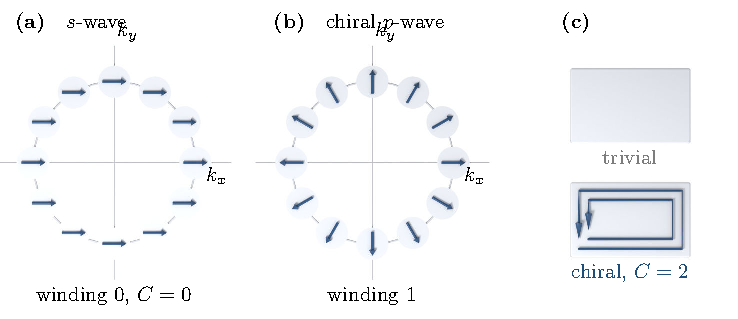
\includegraphics{figures/pdf/s05f04_topology.pdf}
\end{aqmfigure}


\begin{notebookbox}{\texttt{session5.ipynb}, ``Trivial and topological superconducting order parameters, bulk spectra'' (Core), and ``...edge spectra'' (Core)}
Build the s-wave and chiral p-wave BdG Hamiltonians next to each other, and check that their bulk
spectra look similar, since both are gapped with a comparable gap size. Then move to a ribbon
geometry and check that only the p-wave case has gapless chiral edge states, with branches of
opposite velocity on the two edges of the ribbon, which is the distinction driven by the Chern
number of section 5.14.
\end{notebookbox}

\section{Majorana bound states and how to split an electron into two Majoranas}

A \textbf{Majorana fermion} is defined algebraically by the condition that its field operator is
equal to its own Hermitian conjugate,

\begin{equation}
\gamma^\dagger = \gamma,
\end{equation}

which means that the creation and the annihilation of the quasiparticle are the same operation, so
the particle is its own antiparticle. At first this seems to have no place in an ordinary material,
since an ordinary electron is clearly not its own antiparticle ($c^\dagger \ne c$), and a
semiconductor, for example, never hosts anything of this kind.

However, there is a purely algebraic fact that makes it possible. \emph{Any} ordinary fermionic
operator can be written as a combination of two Hermitian Majorana operators that anticommute with
each other,

\begin{equation}
\gamma_A = c + c^\dagger, \qquad \gamma_B = -i\left(c - c^\dagger\right),
\end{equation}

so that $\gamma_A^\dagger = \gamma_A$, $\gamma_B^\dagger = \gamma_B$, $\{\gamma_A,\gamma_B\}=0$ and
$\gamma_A^2=\gamma_B^2=1$, where we used $\{c,c^\dagger\}=1$. If we invert (5.17), we obtain

\begin{equation}
c = \frac{1}{2}\left(\gamma_A + i\gamma_B\right), \qquad c^\dagger = \frac{1}{2}\left(\gamma_A - i\gamma_B\right).
\end{equation}

At first this is only a change of variables, a mathematical trick without new physics. Every
electron is \emph{always} made of two Majorana operators that are tightly bound together into an
ordinary fermion, and normally there is no way to observe $\gamma_A$ or $\gamma_B$ separately, only
their fixed combination $c$. Superconductors are special because BdG eigenstates are already
mixtures of electrons and holes by construction, since the Nambu spinor of section 5.8 explicitly
combines $c_{\mathbf k\sigma}$ with $c_{-\mathbf k\sigma'}^\dagger$. So a superconductor is the
kind of system where, with the right pairing symmetry and the right geometry, the two Majorana
components of an electron can become spatially \emph{separated}, or deconfined, instead of staying
together at one site. This deconfinement is the topic of the rest of this section.

\section{The Kitaev chain as the minimal model with isolated Majoranas}

The simplest superconductor that can host isolated Majoranas is also one of the simplest
superconducting Hamiltonians that we can write, which is a one-dimensional \emph{spinless} chain
with nearest-neighbor hopping and nearest-neighbor pairing,

\begin{equation}
H_{\text{Kitaev}} = -t\sum_n \left(c_n^\dagger c_{n+1} + \text{h.c.}\right) - \mu\sum_n c_n^\dagger c_n + \Delta\sum_n \left(c_n c_{n+1} + c_{n+1}^\dagger c_n^\dagger\right).
\end{equation}

Here the pairing has to be on a bond and not onsite. For spinless fermions, an onsite term $c_n c_n$
vanishes identically because of the Pauli principle ($c_n^2=0$), so the simplest allowed pairing is
the nearest-neighbor term above. After a Fourier transform, the dispersion and the pairing become

\begin{equation}
\varepsilon(k) = -2t\cos k - \mu, \qquad \Delta(k) = 2i\Delta\sin k,
\end{equation}

so the anomalous term is explicitly odd in $k$. As (5.12) already tells us, this means that this is
necessarily a superconductor of spin-triplet type, here a spinless p-wave one, which agrees with the
fact that the onsite channel is forbidden by the Pauli principle.

Now let us set $\mu=0$ and go to the special point $\Delta=t$, and let us substitute the Majorana
decomposition (5.17)-(5.18) at every site, $c_n = \frac{1}{2}(\gamma_{2n-1}+i\gamma_{2n})$. We do
this substitution in both the hopping and the pairing term. The algebra is direct but a bit long,
and it uses the anticommutation relations of the $\gamma$'s, so we suggest that you check it
yourself. The two terms combine so that every $\gamma_{2n-1}\gamma_{2n+2}$ contribution cancels
exactly between hopping and pairing, and the result is very simple,

\begin{equation}
H_{\text{Kitaev}}\Big|_{\Delta=t,\ \mu=0} = it\sum_{n=1}^{N-1} \gamma_{2n}\,\gamma_{2n+1}.
\end{equation}

Every Majorana operator $\gamma_2, \gamma_3, \gamma_4, \dots, \gamma_{2N-1}$ appears in this sum,
paired between neighboring \emph{sites}, but the first Majorana, $\gamma_1$, and the last one,
$\gamma_{2N}$, do not appear at all. They are completely absent from the Hamiltonian, so they cost
zero energy and are completely decoupled from the rest of the system. This is the same structure
that we saw in the SSH model of the topological-band-structure session, in its dimerized
strong-coupling limit. There, at full dimerization, the bulk forms bonding and antibonding dimers,
while one remaining site at each end decouples and gives a zero-energy edge mode. The Kitaev chain
in (5.21) \emph{is} this same structure, written in terms of Majorana operators instead of ordinary
fermion operators, and the two decoupled end Majoranas play the role of the two decoupled end sites
of the SSH model. We do not derive the SSH model again here, and we only recognize it in terms of a
new set of operators. Figure~\ref{fig:s05:kitaev} shows which Majorana is bound to which, in this
phase and in the trivial one.

% Session 5 -- the Kitaev chain: which Majoranas pair with which.
% Placement: sec. "The Kitaev chain", after the SSH-recognition paragraph.
% Rendered by figures/blender/s05f05_kitaev.py, labels in figures/overlays/s05f05_kitaev.tex.
\begin{aqmfigure}{fig:s05:kitaev}{The Kitaev chain in terms of Majorana variables, for $N=5$ sites
(so $\gamma_{2N}=\gamma_{10}$), seen from above. Each site carries two balls, its two Majorana
halves, and a translucent capsule binds two halves together. Splitting every electron into its two
Majorana halves (5.17) has no physical content by itself, and what matters is which halves the
Hamiltonian binds together. In the trivial phase, at the top, the binding is inside each site. The
two halves of each electron stay bound to each other, as they were in the vacuum, and every mode
costs energy. In the topological phase, at the bottom, the binding is between sites, $\gamma_{2n}$
with $\gamma_{2n+1}$, and the pattern has one bond missing at each end. So $\gamma_1$ and
$\gamma_{2N}$ do not appear in (5.21), cost no energy and are at opposite ends of the sample. The
ordinary fermion that they would form together has been split into two halves, which are now
separated by the length of the chain, and this is what \emph{deconfined} means here. This is the
fully dimerized SSH chain of the topological-band-structure session with its two remaining end
sites, with new labels, so the counting is the same and only the operators are new.}
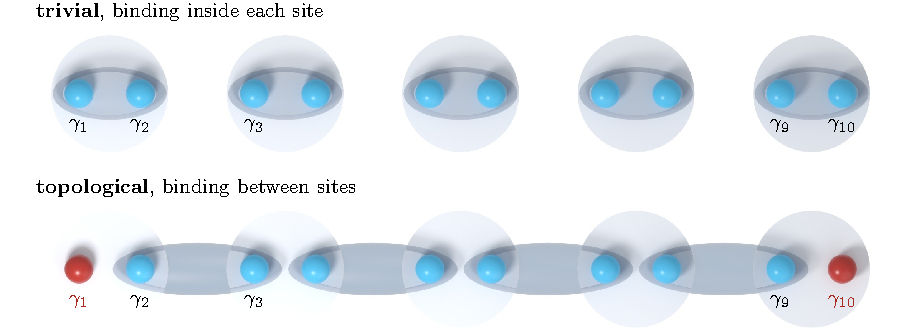
\includegraphics{figures/pdf/s05f05_kitaev.pdf}
\end{aqmfigure}


\begin{notebookbox}{\texttt{session5.ipynb}, ``Emergence of Majorana modes as a function of the size of the superconductor'' (Core)}
Build the Kitaev chain of (5.19), diagonalize it at the fine-tuned point $\Delta=t$, $\mu=0$, and
check directly, as the system size grows, that two states are pinned exactly to zero energy and are
localized at the two ends. These are the two decoupled Majoranas $\gamma_1$ and $\gamma_{2N}$
predicted by (5.21).
\end{notebookbox}

\section{Topological zero modes with periodic and open boundaries}

If we diagonalize (5.19) on a \emph{periodic} chain, we obtain a fully gapped spectrum, with a
superconducting gap set by $\Delta$ and a nontrivial topological invariant of the bulk. This is the
same kind of $\mathbb{Z}_2$ or winding invariant that classified the two phases of the SSH model
through the Zak phase in the topological-band-structure session, now computed from the BdG bands
instead of an ordinary Bloch Hamiltonian. On an \emph{open} chain, for example with $N=100$ sites
and the two ends disconnected, the bulk spectrum keeps essentially the same gap, but two extra
states appear, pinned exactly at zero energy and localized at the left end and at the right end of
the chain. These are the unpaired Majoranas $\gamma_1$
and $\gamma_{2N}$ from (5.21), which we now see as real mid-gap states of the open chain.

These zero modes are very robust. When we move away from the fine-tuned point, with $\Delta \ne t$
and finite $\mu$, the zero modes survive as long as we stay in the same topological phase. The
standard criterion for the general Kitaev chain (5.19) with $\Delta \ne 0$ is

\begin{equation}
|\mu| < 2t \quad \Longrightarrow \quad \text{topological phase (unpaired end Majoranas)}, \qquad |\mu| > 2t \quad \Longrightarrow \quad \text{trivial phase.}
\end{equation}

In the trivial phase, a large chemical potential effectively fixes each site to be either empty or
occupied in the fermionic language, since the chain is spinless, and the two Majoranas that form the electron of each site
combine again locally into an ordinary confined fermion, so nothing is left to deconfine. In the
topological phase, on the other hand, p-wave pairing dominates over the trivial onsite physics, and
the two Majoranas at each site pair with the Majoranas of the neighboring sites instead of with each
other, which leaves the two end Majoranas without any partner. This is the same contrast between
the dimerized strong-coupling limit and the atomic weak-coupling limit that distinguished the
topological and trivial phases of the SSH model. The Kitaev chain reproduces it because, as we saw
in section 5.16, it is the SSH model with new labels.

\section{Engineering a topological superconductor from a quantum spin Hall insulator}

Chiral and p-wave superconductors of the kind we need are rare in nature, so in practice they are
usually \emph{engineered} and not found. One instructive recipe uses directly the quantum spin Hall
(QSH) insulator from the topological-band-structure session. We take a QSH insulator, and the
concrete material used in the lecture is tungsten ditelluride (WTe$_2$), whose edge has helical
modes, meaning that spin-up electrons propagate in one direction and spin-down electrons propagate
in the other direction on the same edge. Now we place ordinary ferromagnets on two segments of this
edge. A magnet breaks time-reversal symmetry locally, and this opens a gap in the helical edge modes
below it. We recall from the topological-band-structure session that the protection of the QSH edge
relies on time-reversal symmetry through Kramers degeneracy, so if we break this symmetry locally,
the protection is lost there. What remains without a gap is a short isolated segment of helical edge
between the two magnetic regions.

This isolated segment only has spin-up electrons moving right and spin-down electrons moving left,
with no spin-down electrons moving right and no spin-up electrons moving left. If we count states
only by their direction of propagation, this segment is \emph{effectively spinless}, which is the
ingredient that the Kitaev-chain construction of section 5.16 needs. If we then couple this segment
by proximity to an ordinary s-wave superconductor, we reproduce on this effectively spinless
one-dimensional system the physics of (5.19), which is a one-dimensional p-wave superconductor with
Majorana zero modes pinned at the two ends of the isolated segment. Figure~\ref{fig:s05:qsh} shows
the whole setup.

% Session 5 -- engineering a Kitaev chain out of a quantum spin Hall edge.
% Placement: sec. "Engineering a topological superconductor from a quantum spin Hall insulator",
% after the proximity-coupling paragraph.
%
% The two Majoranas sit at the ends of the proximitized segment, i.e. exactly at the two
% magnet/superconductor interfaces, per the text.
\begin{aqmfigure}{fig:s05:qsh}{Building the Kitaev chain out of parts that exist. The edge of a
quantum spin Hall insulator is helical: on one and the same edge, spin-up electrons run one way and
spin-down electrons the other. Depositing a ferromagnet on a stretch of that edge breaks
time-reversal symmetry locally and destroys the Kramers protection there, gapping the edge
underneath it; two ferromagnets leave one short helical segment surviving between them. That
segment offers only one propagation direction per spin, so counted as channels it is a
\emph{spinless} one-dimensional wire -- precisely the ingredient (5.19) demands and the one nature
does not hand us directly. Proximity coupling it to an ordinary $s$-wave superconductor supplies
the pairing, and the result is a one-dimensional $p$-wave superconductor carrying a Majorana zero
mode at each end of the segment, that is, at the two ferromagnet--superconductor interfaces. Note
what was \emph{not} required: no unconventional superconductor appears anywhere in the recipe, only
an $s$-wave one, a magnet, and a topological insulator.}

\begin{tikzpicture}[x=1cm, y=1cm]
\tikzset{
  gline/.style={aqm, draw=aqmmuted, line width=0.6pt, dash pattern=on 2pt off 1.5pt},
  chan/.style={aqm, line width=1.1pt, -{Stealth[length=5pt,width=4pt]}},
  majdot/.style={aqm, circle, draw=aqmbroken, fill=aqmfillb, line width=1.1pt,
                 minimum size=10pt, inner sep=0pt}
}

% ============================ the deposited layer ============================
% ferromagnet | superconductor | ferromagnet, all sitting on top of the same edge
\foreach \xa/\xb in {0/4.30, 8.70/13.0} {
  \fill[white] (\xa,2.45) rectangle (\xb,3.35);
  \path[pattern=north east lines, pattern color=aqmmuted] (\xa,2.45) rectangle (\xb,3.35);
  \draw[aqm, draw=aqmmuted] (\xa,2.45) rectangle (\xb,3.35);
  \node[aqmlab, anchor=center, fill=white, inner sep=2.5pt] at ({(\xa+\xb)/2},2.90)
    {ferromagnet};
}
\fill[aqmfill] (4.30,2.45) rectangle (8.70,3.35);
\draw[aqm, draw=aqmaccent] (4.30,2.45) rectangle (8.70,3.35);
\node[aqmlab, anchor=center] at (6.50,2.90) {$s$-wave superconductor};

% ============================ the interfaces =================================
\draw[gline] (4.30,0.36) -- (4.30,2.43);
\draw[gline] (8.70,0.36) -- (8.70,2.43);

% ============================ what each block does ===========================
\node[aqmlabsmall, anchor=north, align=center, text=aqmmuted]
  at (2.15,2.28) {time reversal broken:\\[-2pt]helical modes gapped};
\node[aqmlabsmall, anchor=north, align=center, text=aqmmuted]
  at (10.85,2.28) {time reversal broken:\\[-2pt]helical modes gapped};
\node[aqmlabsmall, anchor=north, align=center]
  at (6.50,2.28) {one direction per spin:\\[-1pt]\textbf{effectively spinless}};

% ============================ the helical edge ===============================
% the surviving segment
\draw[chan, draw=aqmbroken] (4.55,1.15) -- (8.45,1.15);
\node[aqmlabsmall, fill=white, inner sep=1.5pt, text=aqmbroken]
  at (6.50,1.15) {$\uparrow$ moves right};
\draw[chan, draw=aqmbroken] (8.45,0.75) -- (4.55,0.75);
\node[aqmlabsmall, fill=white, inner sep=1.5pt, text=aqmbroken]
  at (6.50,0.75) {$\downarrow$ moves left};
% the gapped stretches
\foreach \xa/\xb in {0.20/4.05, 8.95/12.80} {
  \draw[gline] (\xa,1.15) -- (\xb,1.15);
  \draw[gline] (\xa,0.75) -- (\xb,0.75);
}

% ============================ the slab =======================================
\fill[aqmfill] (0,-1.30) rectangle (13.0,0.36);
\draw[aqm, draw=aqmaccent] (0,-1.30) rectangle (13.0,0.36);
\node[aqmlab, anchor=center] at (6.50,-0.47)
  {quantum spin Hall insulator, gapped bulk \; (e.g.\ WTe$_2$)};

% ============================ the Majoranas ==================================
\node[majdot] at (4.30,0.95) {};
\node[majdot] at (8.70,0.95) {};
\node[aqmlabsmall, anchor=east, text=aqmbroken] at (4.08,0.95) {$\gamma_1$};
\node[aqmlabsmall, anchor=west, text=aqmbroken] at (8.92,0.95) {$\gamma_2$};

% ============================ the read-off ===================================
\node[aqmboxbroken, anchor=north, align=center] at (6.50,-1.60)
  {an effectively spinless 1D segment $+$ proximity pairing $=$ the Kitaev chain (5.19),\\[2pt]
   with its two unpaired end Majoranas now pinned\\[-1pt]
   at the ferromagnet--superconductor interfaces};

\end{tikzpicture}

\end{aqmfigure}


\begin{notebookbox}{\texttt{session5.ipynb}, ``Artificial topological superconductivity'' (Challenge), ``Edge states of an artificial topological superconductor'' (Challenge), and ``Topological phase transition as a function of the exchange field''}
Build the construction described above, with the QSH edge, the magnets and superconductivity, and
check that zero modes localized at the ends emerge as you change the strength of the exchange field.
Look at how the system crosses the boundary between the topological and the trivial phase, of the
type of (5.22), as the magnetic gap changes.
\end{notebookbox}

\section{Topological quantum computing with Majoranas}

Majorana modes get so much attention, beyond their own unusual properties, because of their
proposed use in fault-tolerant quantum computing. Majoranas are \textbf{non-Abelian anyons}.
Exchanging, or braiding, one Majorana around another does not only multiply the many-body ground
state by a phase. It acts as a unitary matrix on a degenerate ground-state manifold, so the
\emph{order} in which different braiding operations are done matters, which means that the algebra
does not commute, and this is what is called non-Abelian. This
follows directly from the structure of the BdG Hamiltonian when more than two Majoranas are present.

For concreteness, four Majorana operators $\gamma_1,\gamma_2,\gamma_3,\gamma_4$ can be combined
again, with pairings of the type of (5.18), into two ordinary fermionic operators, which we can call
artificial fermions, so a system with four Majoranas encodes two ordinary fermionic modes. The
resulting many-body ground-state manifold, with the states empty, one mode filled, the other mode
filled and both filled, is four-fold degenerate. All four states cost zero energy, by the same
argument that made $\gamma_1$ and $\gamma_{2N}$ zero-energy modes in the Kitaev chain, and this
degenerate manifold is the proposed computational basis for a topological qubit.

Braiding two Majoranas, for example $\gamma_1$ around $\gamma_2$, acts on the ground-state manifold
as a unitary

\begin{equation}
U_{12} = \exp\left(\frac{\pi}{4}\,\gamma_1\gamma_2\right),
\end{equation}

which multiplies states by a relative phase built from $e^{i\pi/4}$ times the Majorana product. The
exact form is less important than what it implies. Two exchanges that share a Majorana do not commute.
Braiding the pair $(1,2)$ and then the pair $(2,3)$ gives a different final state than braiding
$(2,3)$ first and $(1,2)$ second, since $\gamma_1\gamma_2$ and $\gamma_2\gamma_3$ anticommute.
Exchanges of disjoint pairs, such as $(1,2)$ and $(3,4)$, commute instead. This braid algebra that does not commute is what allows sequences of
purely topological and geometric moves, which physically means moving Majoranas around one another,
to implement non-trivial quantum logic gates. Since the resulting qubit is stored non-locally,
divided between spatially separated Majoranas instead of being in one local degree of freedom, it is
intrinsically resistant to local decoherence and to weak local disorder, and this robustness is the
main reason for the interest in topological quantum computing. This material on braiding and quantum
computing appears only in the slides and the transcript and has no counterpart in
\texttt{session5.ipynb}. None of the sections of the notebook implement braiding dynamics or a qubit
manifold, which is reasonable, since this is far from a static tight-binding diagonalization and it
is a separate dynamical calculation.

\section{Closing summary}

\begin{itemize}
\item \textbf{Superconductivity is a mean-field, attractive-interaction phenomenon.} Starting from an
attractive Hubbard chain (5.2), pairing mean-field theory gives the order parameter
$\Delta_n = U\langle c_{n\downarrow}c_{n\uparrow}\rangle$ (5.3) and the mean-field Hamiltonian
(5.4).
\item \textbf{Pairing breaks particle-number conservation down to parity} (section 5.6), and this is
the same as the statement that gauge symmetry is spontaneously broken. The pairing term gets a phase
$e^{-2i\varphi}$ under the gauge transformation (5.5), unlike ordinary bilinear terms.
\item \textbf{Flux quantization}, $\Phi = n\, h/2e$ (5.1), is a direct and measurable macroscopic
consequence of this broken gauge symmetry, at the same level as the conductance quantum of the
quantum Hall effect from earlier sessions.
\item \textbf{The Nambu spinor (5.6) and the Bogoliubov-de Gennes Hamiltonian (5.7)-(5.8)} are the
tools that allow us to diagonalize any mean-field superconducting Hamiltonian. They give the
quasiparticle dispersion
$E(\mathbf k) = \pm\sqrt{\varepsilon(\mathbf k)^2 + |\Delta(\mathbf k)|^2}$ (5.9), and a gap opens at
the original Fermi surface regardless of the details of the microscopic dispersion.
\item \textbf{The symmetry of $\Delta(\mathbf k)$ classifies the superconductor.} It can be singlet,
even in $\mathbf
k$, or triplet, odd in $\mathbf k$, as in (5.11)-(5.12), with a further classification by angular
momentum ($L=0,1,2,\dots$) (5.14) that gives s-, p- and d-wave order. The last one is realized in
the cuprate high-$T_c$ superconductors through the nodal $d_{x^2-y^2}$ gap (5.13).
\item \textbf{Gaps with the same spectrum can have different topology.} Trivial s-wave ($C=0$) and
chiral p-wave ($C=\pm2$, eq. 5.15) pairing both fully gap the same Fermi surface, but only the
topological one has gapless edge modes, which is the bulk-boundary logic of the Chern number from
the topological-band-structure and quantum-Hall sessions.
\item \textbf{The Kitaev chain (5.19) is the SSH model in Majorana language.} At the fine-tuned
point it reduces to $H = it\sum_n \gamma_{2n}\gamma_{2n+1}$ (5.21), which leaves two unpaired end
Majoranas with zero energy. These survive away from the fine-tuned point in the whole topological
phase $|\mu|<2t$ (5.22).
\item \textbf{Majoranas are non-Abelian anyons.} Braiding them acts as a unitary (5.23) on a
topologically degenerate ground-state manifold, and exchanges that share a Majorana do not commute, which is the basis of
the proposed schemes for topological quantum computing. This last part is material from the slides
and the transcript, with no counterpart in the notebook.
\end{itemize}

In this session we followed the topic of superconductivity from session 1, from the bare pairing
order parameter to Nambu spinors, Bogoliubov-de Gennes Hamiltonians, the singlet and triplet
classification and finally Majorana zero modes in the Kitaev chain. The division that we made in
session 1 had a second branch that we have not considered since its first short treatment, which is
magnetism, where time-reversal symmetry is broken instead of gauge symmetry. This is where we go
next. Session 6 comes back to the same Hubbard Hamiltonian that opened section 5.5 of this session,
now on its repulsive ($U>0$) side, and gives magnetism the same depth of treatment that we have now
given to superconductivity.
